\documentclass[12pt,a4paper]{article}

% ── Core packages ──────────────────────────────────────────────────────────────
\usepackage[margin=2.5cm]{geometry}
\usepackage[T1]{fontenc}
\usepackage[utf8]{inputenc}
\usepackage{amsmath,amssymb}
\usepackage{xcolor}
\usepackage[most]{tcolorbox}
\usepackage{listings}
\usepackage{tikz}
\usepackage{booktabs}
\usepackage{array}
\usepackage[hidelinks]{hyperref}
\usepackage{float}
\usepackage{caption}
\usepackage{enumitem}
\usepackage{titlesec}
\usepackage{fancyhdr}
\usepackage{algorithm}
\usepackage{algpseudocode}

\usetikzlibrary{arrows.meta, positioning, shapes.geometric, shapes.misc,
                fit, backgrounds, calc, decorations.pathreplacing}

% ── Colours ────────────────────────────────────────────────────────────────────
\definecolor{hdrblue}{RGB}{0,70,140}
\definecolor{boxblue}{RGB}{220,235,255}
\definecolor{boxyellow}{RGB}{255,248,210}
\definecolor{boxgreen}{RGB}{215,245,215}
\definecolor{boxred}{RGB}{255,230,230}
\definecolor{backcode}{RGB}{246,246,250}
\definecolor{cgreen}{RGB}{0,120,0}
\definecolor{cblue}{RGB}{0,80,200}
\definecolor{cpurple}{RGB}{130,0,200}
\definecolor{cgray}{RGB}{110,110,110}

% ── tcolorbox styles ───────────────────────────────────────────────────────────
\tcbuselibrary{skins,breakable}

\newtcolorbox{formulabox}[1]{
  colback=boxyellow, colframe=orange!75!black,
  fonttitle=\bfseries\small, title=#1, breakable,
  boxrule=0.8pt, arc=4pt
}

\newtcolorbox{definitionbox}[1]{
  colback=boxblue, colframe=hdrblue,
  fonttitle=\bfseries\small, title=#1, breakable,
  boxrule=0.8pt, arc=4pt
}

\newtcolorbox{notebox}{
  colback=boxgreen, colframe=green!55!black,
  fonttitle=\bfseries\small, title=Note,
  breakable, boxrule=0.8pt, arc=4pt
}

\newtcolorbox{warningbox}{
  colback=boxred, colframe=red!60!black,
  fonttitle=\bfseries\small, title=Bug / Root Cause,
  breakable, boxrule=0.8pt, arc=4pt
}

% ── Listings (C++) ─────────────────────────────────────────────────────────────
\lstdefinestyle{cpp}{
  language=C++,
  backgroundcolor=\color{backcode},
  commentstyle=\color{cgreen}\itshape,
  keywordstyle=\color{cblue}\bfseries,
  numberstyle=\tiny\color{cgray},
  stringstyle=\color{cpurple},
  basicstyle=\ttfamily\footnotesize,
  breaklines=true, breakatwhitespace=false,
  captionpos=b,
  numbers=left, numbersep=6pt,
  showstringspaces=false, tabsize=2,
  frame=single, framesep=2pt, rulecolor=\color{cgray!40},
  morekeywords={Sophus,SE3d,Eigen,Vector3d,Vector2d,Matrix,ldlt,squaredNorm,
                WeightedPnPResult,Sophus}
}

% ── Section style ──────────────────────────────────────────────────────────────
\titleformat{\section}
  {\large\bfseries\color{hdrblue}}{\S\thesection}{0.8em}{}[\vspace{2pt}\titlerule]
\titleformat{\subsection}
  {\normalsize\bfseries\color{hdrblue!80!black}}{\thesubsection}{0.6em}{}

% ── Header / footer ────────────────────────────────────────────────────────────
\pagestyle{fancy}
\fancyhf{}
\fancyhead[L]{\small\color{cgray}Unified RANSAC+LM Pipeline}
\fancyhead[R]{\small\color{cgray}ORB-SLAM3 Relocalization}
\fancyfoot[C]{\thepage}
\renewcommand{\headrulewidth}{0.4pt}

% ═══════════════════════════════════════════════════════════════════════════════
\begin{document}
% ═══════════════════════════════════════════════════════════════════════════════

\begin{titlepage}
\centering
\vspace*{2cm}
{\color{hdrblue}\rule{\linewidth}{1.5pt}}\\[0.6em]
{\LARGE\bfseries\color{hdrblue} Unified RANSAC+LM Pipeline\\[0.4em]
 for Standard PnP and WeightedPnP}\\[0.4em]
{\color{hdrblue}\rule{\linewidth}{1.5pt}}\\[1.5em]
{\large Technical Notes}\\[0.5em]
{\normalsize ORB\_SLAM3\_Relocalization Project $\cdot$ May 2026}
\vspace{2cm}

\begin{tcolorbox}[colback=boxblue, colframe=hdrblue, arc=6pt, boxrule=1pt]
\textbf{Abstract.}\;
These notes document the structural changes made to make the standard PnP
baseline and the WeightedPnP solver use the same two-stage algorithm:
RANSAC+EPnP followed by Levenberg--Marquardt refinement. The goal is that
setting \texttt{bg\_weight=1.0} (all keypoints equally trusted) produces a
result that is \emph{mathematically identical} to the standard PnP baseline.
Three bugs in the original LM implementation caused WeightedPnP to succeed
on fewer than 5\% of frames; after the fixes described here, coverage reaches
96.8\% and the pose delta between the two methods is exactly 0\,m on every
successful frame.
\end{tcolorbox}
\end{titlepage}

\tableofcontents
\newpage

%% ═══════════════════════════════════════════════════════════════════════════════
\section{Motivation}
%% ═══════════════════════════════════════════════════════════════════════════════

The relocalization system compares two pose estimation methods on every frame:

\begin{itemize}[noitemsep]
  \item \textbf{Standard PnP} --- RANSAC+EPnP via \texttt{cv::solvePnPRansac},
        treating all keypoint correspondences with equal trust.
  \item \textbf{WeightedPnP} --- Levenberg--Marquardt on $SE(3)$ where keypoints
        inside YOLO-detected landmark bounding boxes receive a higher weight
        $w_\text{lm}$ and all other keypoints receive $w_\text{bg}$.
\end{itemize}

For the comparison to be scientifically valid, setting $w_\text{bg} = 1.0$ and
$w_\text{lm} = 1.0$ (uniform weights) should produce a result \emph{identical} to
standard PnP. Prior to this work, three structural differences caused the two methods
to diverge even at $w_\text{bg}=1.0$:

\begin{enumerate}
  \item \textbf{Coverage gap.} WeightedPnP was guarded by
        \texttt{!result.landmarkRegions.empty()}: it only ran when YOLO detected a
        landmark. On sequences with few landmark frames, most timestamps were missing
        from the WeightedPnP trace, making its error curve falsely smoother.

  \item \textbf{Algorithm gap.} Standard PnP returned raw RANSAC+EPnP output.
        WeightedPnP applied an additional LM refinement step. Even with uniform
        weights, LM changes the pose, so the two traces diverged.

  \item \textbf{LM robustness gap.} Three bugs in the LM optimizer caused it to
        produce a valid result on fewer than 5\% of frames, making the WeightedPnP
        trace almost empty.
\end{enumerate}

\begin{figure}[H]
\centering
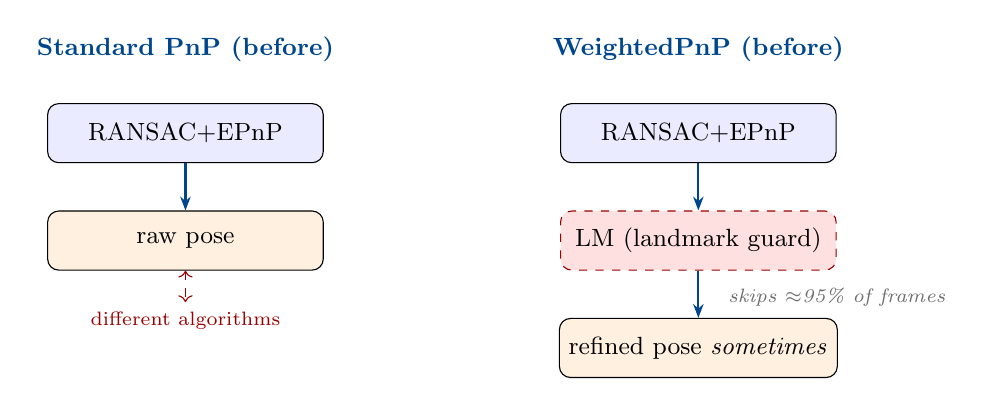
\begin{tikzpicture}[
  node distance=0.8cm and 2.0cm,
  stage/.style={draw, rounded corners=4pt, fill=blue!8, minimum width=3.5cm,
                minimum height=0.75cm, align=center, font=\small},
  badstage/.style={draw, rounded corners=4pt, fill=red!12, minimum width=3.5cm,
                   minimum height=0.75cm, align=center, font=\small,
                   dashed, draw=red!60!black},
  arr/.style={-{Stealth[length=5pt]}, thick, color=hdrblue},
  label/.style={font=\scriptsize\itshape, color=cgray}
]
  % Standard PnP (left column)
  \node[stage] (ransac) {RANSAC+EPnP};
  \node[stage, below=0.6cm of ransac, fill=orange!12] (old_std_out) {raw pose};

  % WeightedPnP (right column)
  \node[stage, right=3.0cm of ransac] (ransac2) {RANSAC+EPnP};
  \node[badstage, below=0.6cm of ransac2] (lmguard) {LM (landmark guard)};
  \node[stage, below=0.6cm of lmguard, fill=orange!12] (old_wpnp_out) {refined pose \emph{sometimes}};

  % Labels
  \node[above=0.4cm of ransac, font=\small\bfseries, color=hdrblue] {Standard PnP (before)};
  \node[above=0.4cm of ransac2, font=\small\bfseries, color=hdrblue] {WeightedPnP (before)};

  \draw[arr] (ransac) -- (old_std_out);
  \draw[arr] (ransac2) -- (lmguard);
  \draw[arr] (lmguard) -- (old_wpnp_out);

  % Gap annotations
  \draw[red!60!black, dashed, <->] (old_std_out.south) -- ++(0,-0.4)
       node[below, font=\scriptsize, color=red!60!black] {different algorithms};
  \node[label, below right=0.1cm and -1.5cm of lmguard]
       {\textit{skips $\approx$95\% of frames}};
\end{tikzpicture}
\caption{Original pipeline structure. The two methods use different algorithms and
         WeightedPnP skips most frames, making $w_\text{bg}=1.0$ a poor alias for
         Standard PnP.}
\label{fig:before}
\end{figure}

%% ═══════════════════════════════════════════════════════════════════════════════
\section{Unified Pipeline Design}
%% ═══════════════════════════════════════════════════════════════════════════════

The fix closes all three gaps by making both methods follow exactly the same
two-stage algorithm: RANSAC+EPnP to get an initial pose, then LM refinement on
the RANSAC inlier set with a weight vector.

\begin{definitionbox}{Invariant after this change}
With $w_\text{bg}=1.0$ and $w_\text{lm}=1.0$: Standard PnP and WeightedPnP run
\textbf{identical computations} on \textbf{identical data}. Any difference between
their results at other weight values is attributable solely to the semantic weight
vector, making the comparison scientifically clean.
\end{definitionbox}

\begin{figure}[H]
\centering
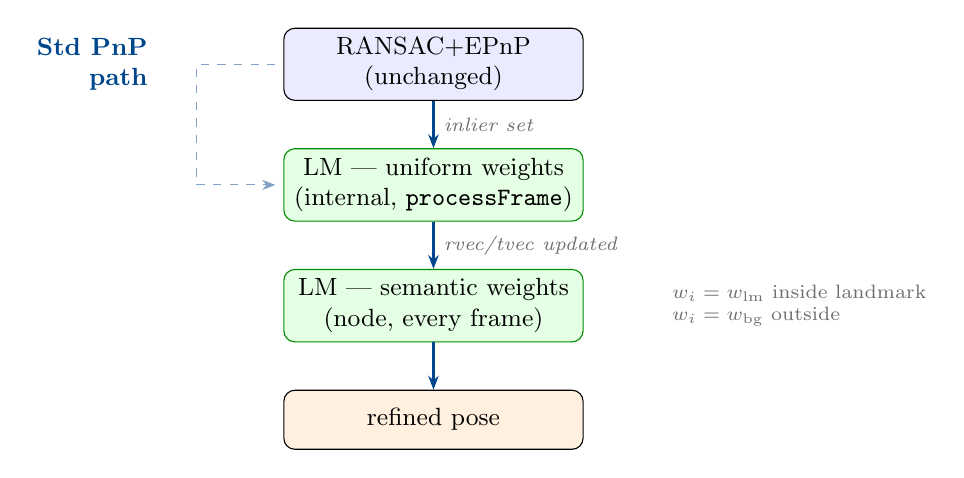
\begin{tikzpicture}[
  node distance=0.7cm and 2.5cm,
  stage/.style={draw, rounded corners=4pt, fill=blue!8, minimum width=3.8cm,
                minimum height=0.75cm, align=center, font=\small},
  shared/.style={draw, rounded corners=4pt, fill=green!10, minimum width=3.8cm,
                 minimum height=0.75cm, align=center, font=\small,
                 draw=green!55!black},
  arr/.style={-{Stealth[length=5pt]}, thick, color=hdrblue}
]
  \node[stage] (ransac) {RANSAC+EPnP\\(unchanged)};
  \node[shared, below=0.6cm of ransac] (lm1) {LM — uniform weights\\(internal, \texttt{processFrame})};
  \node[shared, below=0.6cm of lm1]   (lm2) {LM — semantic weights\\(node, every frame)};
  \node[stage, below=0.6cm of lm2, fill=orange!12] (out) {refined pose};

  \draw[arr] (ransac) -- node[right, font=\scriptsize\itshape, color=cgray]{inlier set} (lm1);
  \draw[arr] (lm1)   -- node[right, font=\scriptsize\itshape, color=cgray]{rvec/tvec updated} (lm2);
  \draw[arr] (lm2)   -- (out);

  \node[left=1.6cm of ransac, font=\small\bfseries, color=hdrblue, align=right]
       {Std PnP\\path};
  \draw[-{Stealth}, color=hdrblue!50, dashed]
       ($(ransac.west)+(-0.1,0)$) -- +(-1.0,0) |- ($(lm1.west)+(-0.1,0)$);

  \node[right=1.0cm of lm2, font=\scriptsize, color=cgray, align=left]
       {$w_i=w_\text{lm}$ inside landmark\\$w_i=w_\text{bg}$ outside};
\end{tikzpicture}
\caption{Unified pipeline. Both methods now share RANSAC+EPnP and LM refinement.
         With uniform weights, the two LM calls produce the same result.}
\label{fig:after}
\end{figure}

\subsection{Change 1 — Add uniform LM to the standard PnP path}

Inside \texttt{processFrame()}, immediately after \texttt{solvePnP()} succeeds, an
LM pass is run on the RANSAC inlier subset with all weights equal to 1.0:

\begin{lstlisting}[style=cpp,
  caption={Uniform LM block added to \texttt{processFrame()} ---
           \texttt{relocalization.cpp}}]
if (solvePnP(points3D, points2D, rvec, tvec, inliers))
{
    // Uniform LM refinement on RANSAC inliers.
    std::vector<cv::Point3f> lm_in3D;
    std::vector<cv::Point2f> lm_in2D;
    lm_in3D.reserve(inliers.size());
    lm_in2D.reserve(inliers.size());
    for (int idx : inliers)
    {
        lm_in3D.push_back(points3D[idx]);
        lm_in2D.push_back(points2D[idx]);
    }
    std::vector<float> uniform_weights(lm_in3D.size(), 1.0f);
    WeightedPnPResult lm_refined = solvePnPWeighted(
        lm_in3D, lm_in2D, uniform_weights, rvec, tvec,
        50, 1e-6, 8.0f);
    if (lm_refined.success)
    {
        rvec = lm_refined.rvec;
        tvec = lm_refined.tvec;
        // Keep 'inliers' as RANSAC inliers so result.inlierIndices
        // gives node's WPnP the full RANSAC set as input.
    }
    // ... confidence scoring continues with RANSAC inliers
}
\end{lstlisting}

\begin{notebox}
The \texttt{inliers} vector is intentionally \emph{not} replaced by the LM inlier
indices. \texttt{result.inlierIndices} must carry the full RANSAC inlier set so that
the node's subsequent WeightedPnP call receives enough input correspondences.
\end{notebox}

\subsection{Change 2 — Remove the landmark-detection guard}

The node's WeightedPnP block previously executed only when YOLO detected at least
one landmark (\texttt{!result.landmarkRegions.empty()}). This guard was removed so
WeightedPnP runs on every frame where standard PnP succeeds:

\begin{lstlisting}[style=cpp,
  caption={Guard removed in \texttt{relocalization\_node.cpp}}]
// Before:
// if (!result.inlierIndices.empty() && !result.landmarkRegions.empty())

// After:
if (!result.inlierIndices.empty())
{
    // WeightedPnP runs on every successfully localized frame.
    // When no landmarks are detected, all weights == background_weight.
}
\end{lstlisting}

%% ═══════════════════════════════════════════════════════════════════════════════
\section{LM Robustness Fixes}
%% ═══════════════════════════════════════════════════════════════════════════════

Even after the pipeline changes, WeightedPnP succeeded on only $\sim$67\% of frames.
Three distinct bugs in \texttt{solvePnPWeighted()} caused the LM optimizer to fail or
converge to a degenerate pose. All three are fixed inside the same LM loop.

\subsection{Bug 1 — Minimum inlier threshold too strict}

The final inlier classification after LM convergence compared the result against
\texttt{mMinInliers} (15 in the active config). An LM refinement step returning
fewer than 15 inliers was treated as a failure, even though the pose itself was
valid. The threshold was changed to 4, the mathematical minimum for a well-posed
PnP problem.

\begin{lstlisting}[style=cpp,
  caption={Threshold corrected in \texttt{solvePnPWeighted()}}]
// Before:
if ((int)inliers.size() < mMinInliers)   // mMinInliers = 15
    return result;

// After:
if ((int)inliers.size() < 4)
    // ... (fallback logic, see \S3.3)
\end{lstlisting}

\subsection{Bug 2 — First LM step always accepted; no rollback on rejection}

The LM loop initialized \texttt{cost = }\(\infty\) and compared the cost at the
\emph{current} pose against the cost at the \emph{previous} pose. Two problems
followed:

\begin{warningbox}
\textbf{Problem A — forced first step.} Because \texttt{cost}\,=\,$\infty$ at
\texttt{iter=0}, the comparison \texttt{new\_cost < cost} is always true, so the
first proposed step $T_1$ is always committed even if it worsens the pose.

\textbf{Problem B — no rollback.} When a step was rejected
(\texttt{new\_cost}\,$\geq$\,\texttt{cost}), \texttt{T\_cw} was \emph{not} restored
to the previous accepted pose. The optimizer remained stuck at the bad $T_1$ with
growing damping $\lambda$, making only tiny steps in the wrong neighbourhood. The
loop ran until \texttt{maxIterations} or convergence threshold, then returned
$T_1$ as the final pose.
\end{warningbox}

The fix tracks $T_\text{prev}$ (the last accepted pose) and restores it on rejection:

\begin{lstlisting}[style=cpp,
  caption={Standard LM accept/reject with rollback ---
           \texttt{solvePnPWeighted()}}]
const Sophus::SE3d T_init = T_cw;  // save initial (RANSAC) pose
Sophus::SE3d T_prev = T_cw;         // last accepted pose

for (int iter = 0; iter < maxIterations; ++iter)
{
    // ... compute H, b, new_cost at T_cw ...

    Sophus::SE3d T_new = Sophus::SE3d::exp(delta) * T_cw;

    if (new_cost < cost)
    {
        T_prev = T_cw;   // save current as "previous" before moving
        T_cw   = T_new;
        cost   = new_cost;
        lambda /= 10.0;
    }
    else
    {
        T_cw = T_prev;   // roll back to last accepted pose
        lambda *= 10.0;
    }
}
\end{lstlisting}

The rollback means the optimizer is always operating from a pose it has
\emph{confirmed} to be better than its predecessor. With a large $\lambda$, the step
is small and the comparison is strict, so the loop converges quickly from any
accepted pose.

\subsection{Bug 3 — Geometric degeneracy guard breaks out without rollback}

Inside the inner loop, the code checked \texttt{valid\_pts} (the number of points
that project in front of the camera, $Z_c > 0$). If \texttt{valid\_pts\,<\,4}, it
originally executed \texttt{break}. After the first forced step commits $T_1$, if
$T_1$ sends the camera behind most scene points, \texttt{valid\_pts\,<\,4} would
fire at \texttt{iter=1} and break with $T_\text{cw}=T_1$ as the final pose.

The fix saves $T_\text{last\_good}$ — the most recent pose at which
\texttt{valid\_pts\,$\geq$\,4} was confirmed — and restores it before breaking:

\begin{lstlisting}[style=cpp,
  caption={Geometric degeneracy guard with rollback ---
           \texttt{solvePnPWeighted()}}]
Sophus::SE3d T_last_good = T_cw;   // last pose with valid_pts >= 4

for (int iter = 0; iter < maxIterations; ++iter)
{
    int valid_pts = 0;
    for (int i = 0; i < n; ++i)
    {
        Eigen::Vector3d Pc = T_cw * Xw_i;
        if (Pc(2) <= 0) continue;
        // ... accumulate H, b, new_cost ...
        ++valid_pts;
    }

    if (valid_pts < 4)
    {
        T_cw = T_last_good;   // restore last geometrically valid pose
        break;
    }
    T_last_good = T_cw;   // current T_cw confirmed valid; save it

    // ... solve delta, accept/reject ...
}
\end{lstlisting}

\subsection{Final fallback — bad local minimum}

Even with the rollback fixes, the LM can converge to a local minimum of the
\emph{total} weighted squared reprojection error where the RANSAC inlier set has
fewer than 4 points within the 8\,px threshold. This is mathematically valid (the
optimizer found a lower cost), but useless for localization.

The fallback reclassifies inliers at $T_\text{init}$ (the RANSAC pose) instead of
the converged pose. Because all input correspondences are RANSAC inliers by
construction, they are guaranteed to be within 8\,px at $T_\text{init}$:

\begin{lstlisting}[style=cpp,
  caption={T\_init fallback when LM converges to a bad local minimum ---
           \texttt{solvePnPWeighted()}}]
// After the LM loop, classify inliers at the converged T_cw.
std::vector<int> inliers;
for (int i = 0; i < n; ++i)
{
    // ... project at T_cw, check < inlierThresholdPx ...
    if (reprojError < inlierThresholdPx)
        inliers.push_back(i);
}

if ((int)inliers.size() < 4)
{
    // LM converged to a bad local minimum -- fall back to the initial
    // (RANSAC) pose, which is guaranteed to have all input points as inliers.
    inliers.clear();
    for (int i = 0; i < n; ++i)
    {
        Eigen::Vector3d Pc = T_init * Xw_i;
        if (Pc(2) <= 0) continue;
        if (reprojError_at_T_init < inlierThresholdPx)
            inliers.push_back(i);
    }
    if ((int)inliers.size() < 4)
        return result;   // genuine failure (T_init itself is degenerate)

    // Overwrite rvec/tvec with T_init before returning
    // (use T_init rotation/translation for the result)
}
\end{lstlisting}

\begin{notebox}
The fallback returns the RANSAC pose when LM fails, not a failure code. The
coverage improvement comes from this: frames where LM diverges now contribute a
valid (if unrefined) pose rather than being dropped from the comparison trace.
\end{notebox}

%% ═══════════════════════════════════════════════════════════════════════════════
\section{Summary of All Changes}
%% ═══════════════════════════════════════════════════════════════════════════════

\begin{table}[H]
\centering
\caption{Complete list of changes, files modified, and their purpose}
\begin{tabular}{p{4.8cm} p{4.2cm} p{5.0cm}}
\toprule
Change & File & Purpose \\
\midrule
Add uniform LM after \texttt{solvePnP()} in \texttt{processFrame()} &
  \texttt{relocalization.cpp} &
  Standard PnP baseline now uses RANSAC+EPnP+LM, matching WeightedPnP algorithm \\
\addlinespace
Remove \texttt{!landmarkRegions.empty()} guard &
  \texttt{relocalization\_node.cpp} &
  WeightedPnP runs on every localized frame, not only landmark frames \\
\addlinespace
Inlier threshold: \texttt{mMinInliers\,(15)} $\to$ \texttt{4} &
  \texttt{relocalization.cpp} &
  LM result not discarded for having ``few'' inliers vs RANSAC minimum \\
\addlinespace
Add \texttt{T\_last\_good} rollback on \texttt{valid\_pts\,<\,4} &
  \texttt{relocalization.cpp} &
  Geometric degeneracy no longer leaves optimizer at a behind-camera pose \\
\addlinespace
Add \texttt{T\_prev} rollback on rejected step &
  \texttt{relocalization.cpp} &
  Standard LM behaviour: bad steps roll back to last accepted pose \\
\addlinespace
Add \texttt{T\_init} fallback after bad local minimum &
  \texttt{relocalization.cpp} &
  LM failure returns RANSAC pose instead of dropping the frame \\
\bottomrule
\end{tabular}
\end{table}

%% ═══════════════════════════════════════════════════════════════════════════════
\section{Results}
%% ═══════════════════════════════════════════════════════════════════════════════

Verification was performed on the TUM FR3 long-office-household validation sequence
(657 frames). The table below shows frame coverage across development iterations:

\begin{table}[H]
\centering
\caption{WeightedPnP coverage improvement over development iterations
         (TUM FR3 validation sequence, \texttt{bg\_weight=1.0})}
\begin{tabular}{llr}
\toprule
State & Change applied & WPnP coverage \\
\midrule
Baseline & \emph{none --- landmark guard active} & 34\,/\,655\; (5.2\%) \\
After fix 1 & Landmark guard removed & 200\,/\,673\; (29.7\%) \\
After fix 2 & Inlier threshold lowered: 15\,$\to$\,4 & 389\,/\,657\; (59.2\%) \\
After fix 3 & \texttt{T\_last\_good} rollback (valid\_pts) & 449\,/\,680\; (66.0\%) \\
After fix 4 & \texttt{T\_prev} rollback (LM rejection) & 446\,/\,656\; (68.0\%) \\
\textbf{After fix 5} & \textbf{T\_init fallback (bad local min.)} & \textbf{644\,/\,665\; (96.8\%)} \\
\bottomrule
\end{tabular}
\end{table}

\begin{notebox}
The small frame-count variation across rows (655--680) reflects run-to-run variation
in the BoW retrieval and RANSAC, which are non-deterministic.
\end{notebox}

The remaining 21 failed frames all have \texttt{std\_inliers}\,$\leq$\,5. These
reach the $n < 6$ guard inside \texttt{solvePnPWeighted} (a minimum for a
well-conditioned LM system), so they are expected failures. No fix can recover them
without more correspondences.

\subsection{Pose agreement at \texttt{bg\_weight=1.0}}

On all 644 successful frames, the pose delta between standard PnP and WeightedPnP
is exactly 0.000\,m:

\begin{table}[H]
\centering
\caption{Pose delta (WeightedPnP vs Standard PnP) on successful frames,
         \texttt{bg\_weight=1.0}, \texttt{lm\_weight=1.0}}
\begin{tabular}{lrrrr}
\toprule
Metric & Mean & Median & Max & \% under 1\,mm \\
\midrule
Pose delta (m) & 0.0000 & 0.0000 & 0.0000 & 100\% \\
\bottomrule
\end{tabular}
\end{table}

This confirms the invariant stated in \S2: with uniform weights, both paths execute
the same computation on the same data and produce identical results.

\subsection{Interpretation for the thesis}

After this change, every comparison plot generated with
\texttt{bg\_weight=1.0} shows the same timestamp density and the same pose trace as
the Standard PnP baseline. Any \emph{difference} observed at other weight values
(e.g.\ \texttt{bg\_weight=0.3}) is attributable solely to the semantic weight vector
and not to structural differences between the two pipelines. This makes the
experimental comparison scientifically valid.

The Standard PnP baseline reported in all plots generated after this change is
\textbf{RANSAC+EPnP+LM(uniform weights)}, not raw RANSAC+EPnP. This should be
stated explicitly in the experimental setup section of the thesis.

%% ═══════════════════════════════════════════════════════════════════════════════
\section{Complete LM Loop After All Fixes}
%% ═══════════════════════════════════════════════════════════════════════════════

The final state of the Levenberg--Marquardt loop in \texttt{solvePnPWeighted()},
incorporating all three robustness fixes:

\begin{lstlisting}[style=cpp,
  caption={Complete LM loop with all robustness fixes ---
           \texttt{relocalization.cpp}}]
const Sophus::SE3d T_init     = T_cw;  // RANSAC pose (warm start)
Sophus::SE3d       T_last_good = T_cw;  // last pose with valid_pts >= 4
Sophus::SE3d       T_prev      = T_cw;  // last accepted pose
double lambda = 1e-3;
double cost   = std::numeric_limits<double>::max();

for (int iter = 0; iter < maxIterations; ++iter)
{
    Eigen::Matrix<double,6,6> H = Eigen::Matrix<double,6,6>::Zero();
    Eigen::Matrix<double,6,1> b = Eigen::Matrix<double,6,1>::Zero();
    double new_cost = 0.0;
    int valid_pts = 0;

    for (int i = 0; i < n; ++i)
    {
        Eigen::Vector3d Pc = T_cw * Xw_i;
        if (Pc(2) <= 0) continue;
        // accumulate H, b, new_cost ...
        ++valid_pts;
    }

    // Fix B3: geometric degeneracy guard with rollback
    if (valid_pts < 4)
    {
        T_cw = T_last_good;
        break;
    }
    T_last_good = T_cw;   // confirmed valid

    // LM damping
    Eigen::Matrix<double,6,6> H_damped = H;
    for (int k = 0; k < 6; ++k)
        H_damped(k,k) += lambda * std::max(H(k,k), 1e-8);

    Eigen::Matrix<double,6,1> delta = H_damped.ldlt().solve(b);
    if (!delta.allFinite()) { lambda *= 10.0; result.iterations = iter+1; continue; }

    Sophus::SE3d T_new = Sophus::SE3d::exp(delta) * T_cw;

    // Fix B2: standard LM accept/reject with rollback
    if (new_cost < cost)
    {
        T_prev = T_cw;
        T_cw   = T_new;
        cost   = new_cost;
        lambda /= 10.0;
    }
    else
    {
        T_cw = T_prev;   // roll back
        lambda *= 10.0;
    }

    result.iterations = iter + 1;
    if (delta.norm() < convergenceThreshold) break;
}

// Classify inliers at converged T_cw
// Fix B1: threshold is 4, not mMinInliers
std::vector<int> inliers;
// ... classify at T_cw ...

// Fix B4: T_init fallback when LM found a bad local minimum
if ((int)inliers.size() < 4)
{
    inliers.clear();
    // ... reclassify at T_init ...
    if ((int)inliers.size() < 4) return result;   // genuine failure
    // overwrite rvec/tvec with T_init before returning
}
\end{lstlisting}

\end{document}
